\documentclass{standalone}
\usepackage{tikz}
\usetikzlibrary{patterns, positioning}


\begin{document}
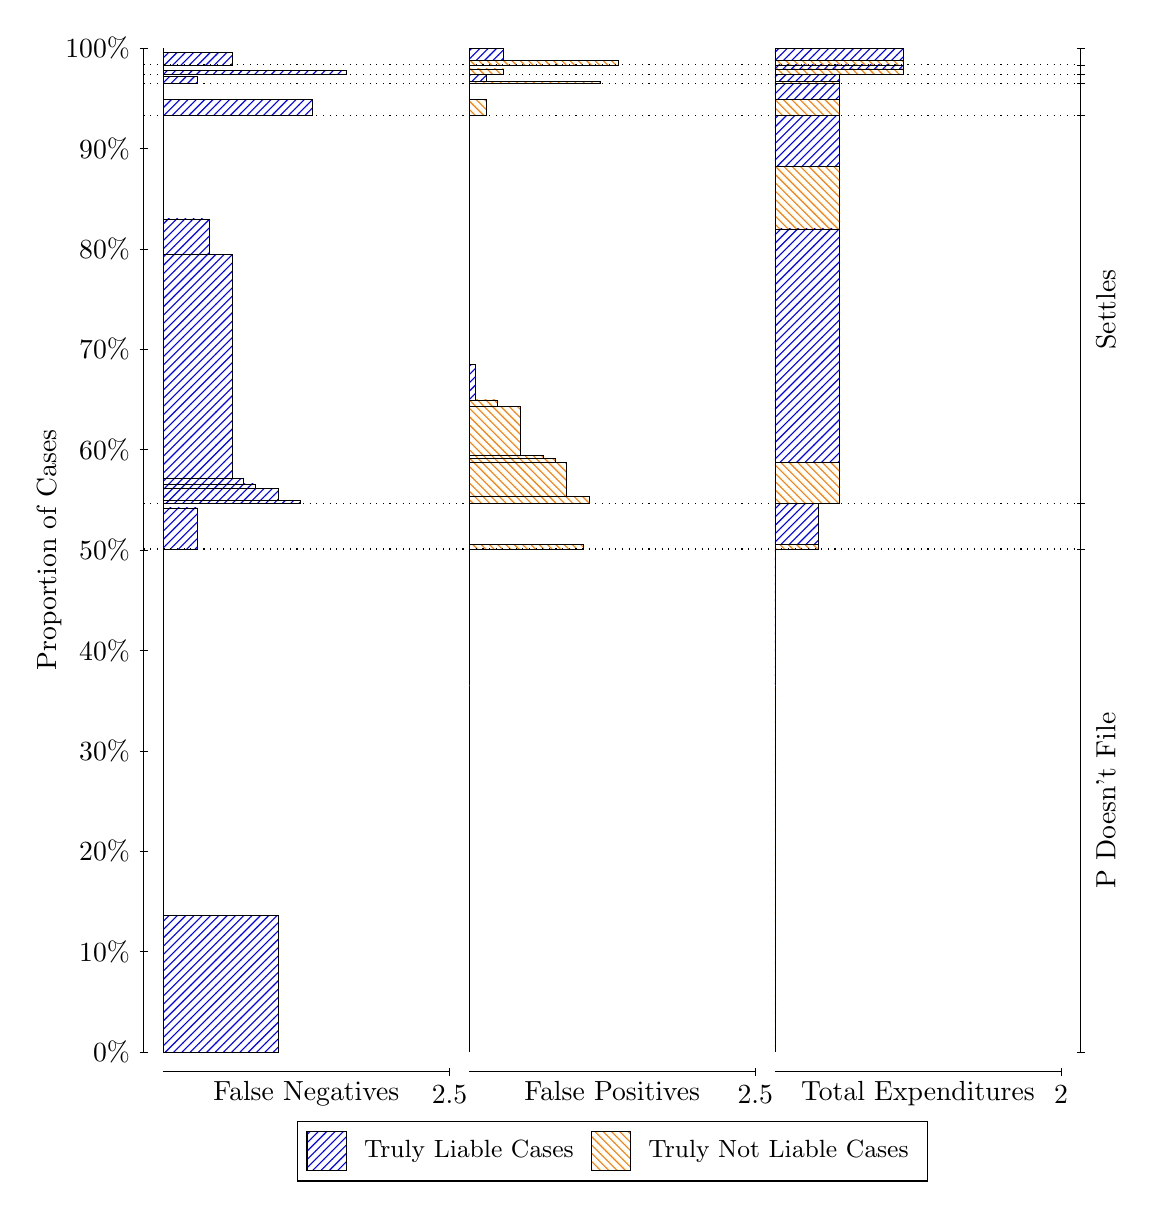
\begin{tikzpicture}
\draw[black, very thin] (1.5,1.75) -- (1.5,14.5);
\node[rotate=90, text=black, anchor=center] at (0.3, 8.125) {Proportion of Cases};
\draw[black, very thin] (1.45,1.75) -- (1.55,1.75);
\node[text=black, anchor=east] at (1.45, 1.75) {0\%};
\draw[black, very thin] (1.45,3.025) -- (1.55,3.025);
\node[text=black, anchor=east] at (1.45, 3.025) {10\%};
\draw[black, very thin] (1.45,4.3) -- (1.55,4.3);
\node[text=black, anchor=east] at (1.45, 4.3) {20\%};
\draw[black, very thin] (1.45,5.575) -- (1.55,5.575);
\node[text=black, anchor=east] at (1.45, 5.575) {30\%};
\draw[black, very thin] (1.45,6.85) -- (1.55,6.85);
\node[text=black, anchor=east] at (1.45, 6.85) {40\%};
\draw[black, very thin] (1.45,8.125) -- (1.55,8.125);
\node[text=black, anchor=east] at (1.45, 8.125) {50\%};
\draw[black, very thin] (1.45,9.4) -- (1.55,9.4);
\node[text=black, anchor=east] at (1.45, 9.4) {60\%};
\draw[black, very thin] (1.45,10.675) -- (1.55,10.675);
\node[text=black, anchor=east] at (1.45, 10.675) {70\%};
\draw[black, very thin] (1.45,11.95) -- (1.55,11.95);
\node[text=black, anchor=east] at (1.45, 11.95) {80\%};
\draw[black, very thin] (1.45,13.225) -- (1.55,13.225);
\node[text=black, anchor=east] at (1.45, 13.225) {90\%};
\draw[black, very thin] (1.45,14.5) -- (1.55,14.5);
\node[text=black, anchor=east] at (1.45, 14.5) {100\%};

\draw[black, very thin] (13.4,1.75) -- (13.4,14.5);
\draw[black, very thin] (13.35,1.75) -- (13.45,1.75);
\node[anchor=west] at (13.35, 1.75) {};
\draw[black, very thin] (13.35,8.1374) -- (13.45,8.1374);
\node[anchor=west] at (13.35, 8.1374) {};
\draw[black, very thin] (13.35,8.7166) -- (13.45,8.7166);
\node[anchor=west] at (13.35, 8.7166) {};
\draw[black, very thin] (13.35,13.644) -- (13.45,13.644);
\node[anchor=west] at (13.35, 13.644) {};
\draw[black, very thin] (13.35,14.047) -- (13.45,14.047);
\node[anchor=west] at (13.35, 14.047) {};
\draw[black, very thin] (13.35,14.166) -- (13.45,14.166);
\node[anchor=west] at (13.35, 14.166) {};
\draw[black, very thin] (13.35,14.287) -- (13.45,14.287);
\node[anchor=west] at (13.35, 14.287) {};
\draw[black, very thin] (13.35,14.5) -- (13.45,14.5);
\node[anchor=west] at (13.35, 14.5) {};

\draw[black, very thin, pattern color=blue, pattern=north east lines] (1.75,1.75) rectangle (3.2033,3.4862);
\draw[black, very thin, pattern color=orange, pattern=north west lines] (1.75,3.4862) rectangle (1.75,8.1374);
\draw[black, very thin, pattern color=blue, pattern=north east lines] (1.75,8.1374) rectangle (2.186,8.6589);
\draw[black, very thin, pattern color=orange, pattern=north west lines] (1.75,8.6589) rectangle (1.75,8.7166);
\draw[black, very thin, pattern color=blue, pattern=north east lines] (1.75,8.7166) rectangle (3.494,8.7511);
\draw[black, very thin, pattern color=blue, pattern=north east lines] (1.75,8.7511) rectangle (3.2033,8.9045);
\draw[black, very thin, pattern color=blue, pattern=north east lines] (1.75,8.9045) rectangle (2.9127,8.9654);
\draw[black, very thin, pattern color=blue, pattern=north east lines] (1.75,8.9654) rectangle (2.7673,9.0371);
\draw[black, very thin, pattern color=blue, pattern=north east lines] (1.75,9.0371) rectangle (2.622,11.875);
\draw[black, very thin, pattern color=blue, pattern=north east lines] (1.75,11.875) rectangle (2.3313,12.33);
\draw[black, very thin, pattern color=orange, pattern=north west lines] (1.75,12.33) rectangle (1.75,13.644);
\draw[black, very thin, pattern color=blue, pattern=north east lines] (1.75,13.644) rectangle (3.6393,13.847);
\draw[black, very thin, pattern color=orange, pattern=north west lines] (1.75,13.847) rectangle (1.75,14.047);
\draw[black, very thin, pattern color=blue, pattern=north east lines] (1.75,14.047) rectangle (2.186,14.135);
\draw[black, very thin, pattern color=orange, pattern=north west lines] (1.75,14.135) rectangle (1.75,14.166);
\draw[black, very thin, pattern color=blue, pattern=north east lines] (1.75,14.166) rectangle (4.0753,14.218);
\draw[black, very thin, pattern color=orange, pattern=north west lines] (1.75,14.218) rectangle (1.75,14.287);
\draw[black, very thin, pattern color=blue, pattern=north east lines] (1.75,14.287) rectangle (2.622,14.447);
\draw[black, very thin, pattern color=orange, pattern=north west lines] (1.75,14.447) rectangle (1.75,14.5);
\draw[black, very thin, pattern color=orange, pattern=north west lines] (5.6333,1.75) rectangle (5.6333,6.4012);
\draw[black, very thin, pattern color=blue, pattern=north east lines] (5.6333,6.4012) rectangle (5.6333,8.1374);
\draw[black, very thin, pattern color=orange, pattern=north west lines] (5.6333,8.1374) rectangle (7.0867,8.1951);
\draw[black, very thin, pattern color=blue, pattern=north east lines] (5.6333,8.1951) rectangle (5.6333,8.7166);
\draw[black, very thin, pattern color=orange, pattern=north west lines] (5.6333,8.7166) rectangle (7.1593,8.8092);
\draw[black, very thin, pattern color=orange, pattern=north west lines] (5.6333,8.8092) rectangle (6.8687,9.2377);
\draw[black, very thin, pattern color=orange, pattern=north west lines] (5.6333,9.2377) rectangle (6.7233,9.2859);
\draw[black, very thin, pattern color=orange, pattern=north west lines] (5.6333,9.2859) rectangle (6.578,9.3256);
\draw[black, very thin, pattern color=orange, pattern=north west lines] (5.6333,9.3256) rectangle (6.2873,9.9525);
\draw[black, very thin, pattern color=orange, pattern=north west lines] (5.6333,9.9525) rectangle (5.9967,10.031);
\draw[black, very thin, pattern color=blue, pattern=north east lines] (5.6333,10.031) rectangle (5.706,10.485);
\draw[black, very thin, pattern color=blue, pattern=north east lines] (5.6333,10.485) rectangle (5.6333,13.644);
\draw[black, very thin, pattern color=orange, pattern=north west lines] (5.6333,13.644) rectangle (5.8513,13.844);
\draw[black, very thin, pattern color=blue, pattern=north east lines] (5.6333,13.844) rectangle (5.6333,14.047);
\draw[black, very thin, pattern color=orange, pattern=north west lines] (5.6333,14.047) rectangle (7.3047,14.078);
\draw[black, very thin, pattern color=blue, pattern=north east lines] (5.6333,14.078) rectangle (5.8513,14.166);
\draw[black, very thin, pattern color=orange, pattern=north west lines] (5.6333,14.166) rectangle (6.0693,14.234);
\draw[black, very thin, pattern color=blue, pattern=north east lines] (5.6333,14.234) rectangle (5.6333,14.287);
\draw[black, very thin, pattern color=orange, pattern=north west lines] (5.6333,14.287) rectangle (7.5227,14.339);
\draw[black, very thin, pattern color=blue, pattern=north east lines] (5.6333,14.339) rectangle (6.0693,14.5);
\draw[black, very thin, pattern color=orange, pattern=north west lines] (9.5167,1.75) rectangle (9.5167,6.4012);
\draw[black, very thin, pattern color=blue, pattern=north east lines] (9.5167,6.4012) rectangle (9.5167,8.1374);
\draw[black, very thin, pattern color=orange, pattern=north west lines] (9.5167,8.1374) rectangle (10.062,8.1951);
\draw[black, very thin, pattern color=blue, pattern=north east lines] (9.5167,8.1951) rectangle (10.062,8.7166);
\draw[black, very thin, pattern color=orange, pattern=north west lines] (9.5167,8.7166) rectangle (10.334,9.233);
\draw[black, very thin, pattern color=blue, pattern=north east lines] (9.5167,9.233) rectangle (10.334,12.204);
\draw[black, very thin, pattern color=orange, pattern=north west lines] (9.5167,12.204) rectangle (10.334,13.001);
\draw[black, very thin, pattern color=blue, pattern=north east lines] (9.5167,13.001) rectangle (10.334,13.644);
\draw[black, very thin, pattern color=orange, pattern=north west lines] (9.5167,13.644) rectangle (10.334,13.844);
\draw[black, very thin, pattern color=blue, pattern=north east lines] (9.5167,13.844) rectangle (10.334,14.047);
\draw[black, very thin, pattern color=orange, pattern=north west lines] (9.5167,14.047) rectangle (10.334,14.078);
\draw[black, very thin, pattern color=blue, pattern=north east lines] (9.5167,14.078) rectangle (10.334,14.166);
\draw[black, very thin, pattern color=orange, pattern=north west lines] (9.5167,14.166) rectangle (11.152,14.234);
\draw[black, very thin, pattern color=blue, pattern=north east lines] (9.5167,14.234) rectangle (11.152,14.287);
\draw[black, very thin, pattern color=orange, pattern=north west lines] (9.5167,14.287) rectangle (11.152,14.339);
\draw[black, very thin, pattern color=blue, pattern=north east lines] (9.5167,14.339) rectangle (11.152,14.5);
\draw[black, dotted] (1.5,8.1374) -- (13.4,8.1374);
\draw[black, dotted] (1.5,8.7166) -- (13.4,8.7166);
\draw[black, dotted] (1.5,13.644) -- (13.4,13.644);
\draw[black, dotted] (1.5,14.047) -- (13.4,14.047);
\draw[black, dotted] (1.5,14.166) -- (13.4,14.166);
\draw[black, dotted] (1.5,14.287) -- (13.4,14.287);
\draw[black, very thin] (1.75,1.5) -- (5.3833,1.5);
\node[text=black, anchor=north] at (3.5667, 1.5) {False Negatives};
\draw[black, very thin] (5.3833,1.45) -- (5.3833,1.55);
\node[text=black, anchor=north] at (5.3833, 1.45) {2.5};

\draw[black, very thin] (5.6333,1.5) -- (9.2667,1.5);
\node[text=black, anchor=north] at (7.45, 1.5) {False Positives};
\draw[black, very thin] (9.2667,1.45) -- (9.2667,1.55);
\node[text=black, anchor=north] at (9.2667, 1.45) {2.5};

\draw[black, very thin] (9.5167,1.5) -- (13.15,1.5);
\node[text=black, anchor=north] at (11.333, 1.5) {Total Expenditures};
\draw[black, very thin] (13.15,1.45) -- (13.15,1.55);
\node[text=black, anchor=north] at (13.15, 1.45) {2};

\node[text=black, centered, rotate=90] at (13.72, 4.9437) {P Doesn't File};

\node[text=black, centered, rotate=90] at (13.72, 11.18) {Settles};





\draw (7.449999999999999,1.5) node[draw=none] (baseCoordinate) {};
\begin{scope}[align=center]
        \matrix[scale=0.5, draw=black, below=0.5cm of baseCoordinate, nodes={draw}, column sep=0.1cm]{
            \node[rectangle, draw, minimum width=0.5cm, minimum height=0.5cm, pattern color=blue, pattern=north east lines] {}; &
            \node[draw=none, font=\small, text=black] (B) {Truly Liable Cases}; &
            \node[rectangle, draw, minimum width=0.5cm, minimum height=0.5cm, pattern color=orange, pattern=north west lines] {}; &
            \node[draw=none, font=\small, text=black] (B) {Truly Not Liable Cases}; \\
            };
\end{scope}

\end{tikzpicture}
\end{document}